\documentclass[a4paper, fontsize=14pt]{article}
\usepackage[T2A]{fontenc}
\usepackage{mathtools}
\usepackage[utf8]{inputenc}
\usepackage[english, russian]{babel}
\usepackage{fancyhdr}
\usepackage{graphicx}
\usepackage{gensymb}
\usepackage{floatrow}
\usepackage{titlesec}
\usepackage{lastpage}
\usepackage{float}
\usepackage{gensymb}
\usepackage{booktabs}
\usepackage{amsmath}
\usepackage{amssymb}

\pagestyle{fancy}
	\fancyhf{}
	\lhead{\hspace{1bp} Работа \textnumero 4.1.2}
	\rhead{Терехов Максим 876\hspace{1bp}}
	\lfoot{Измерение магнитного поля Земли}
	\cfoot{\textbf{}}
	\rfoot{\thepage\ \textnormal{из}\ \pageref{LastPage}}
	\renewcommand{\headrulewidth}{1pt}
	\renewcommand{\footrulewidth}{1pt}


%\addtolength{\hoffset}{-1.75cm}
%\addtolength{\textwidth}{3.5cm} 

%\addtolength{\voffset}{-1.5cm}
%\addtolength{\textheight}{3cm} 

\titleformat{\section}
    [block]{\normalfont\bfseries\large}{\rlap{\thesection}}{0em}
    {\vspace{-0.02\textwidth}\begin{minipage}[t]{.95\textwidth}}
[\end{minipage}]

\thispagestyle{fancy}

\begin{document}
\selectlanguage{russian}


\huge
\centering
\textbf{Измерение магнитного поля Земли}

\raggedright
\parindent=1cm
\large
	\section*{Цель работы}
	Определить характеристики шарообразных неодимовых магнитов и, используя законы взаимодействия магнитных моментов с полем, измерить горизонтальную и вертикальную составляющие индукции магнитного поля Земли и магнитное наклонение.
	\section*{Оборудование}
	12 одинаковых неодимовых магнитных шариков, тонкая нить для изготовления крутильного маятника, медная проволока диаметром (0,5 --- 0,6) мм, электронные весы, секундомер, измеритель магнитной индукции АТЕ-8702, штангенциркуль, брусок из немагнитного материала  (25$\times$ 30$\times$ 60  $\text{мм}^3$), деревянная  линейка, штатив из  немагнитного  материала; дополнительные неодимовые магнитные шарики (~ 20 шт.) и неодимовые магниты в форме параллелепипедов (2 шт.), набор гирь и разновесов.
	\section*{Экспериментальная установка}
		\begin{figure}[H]
	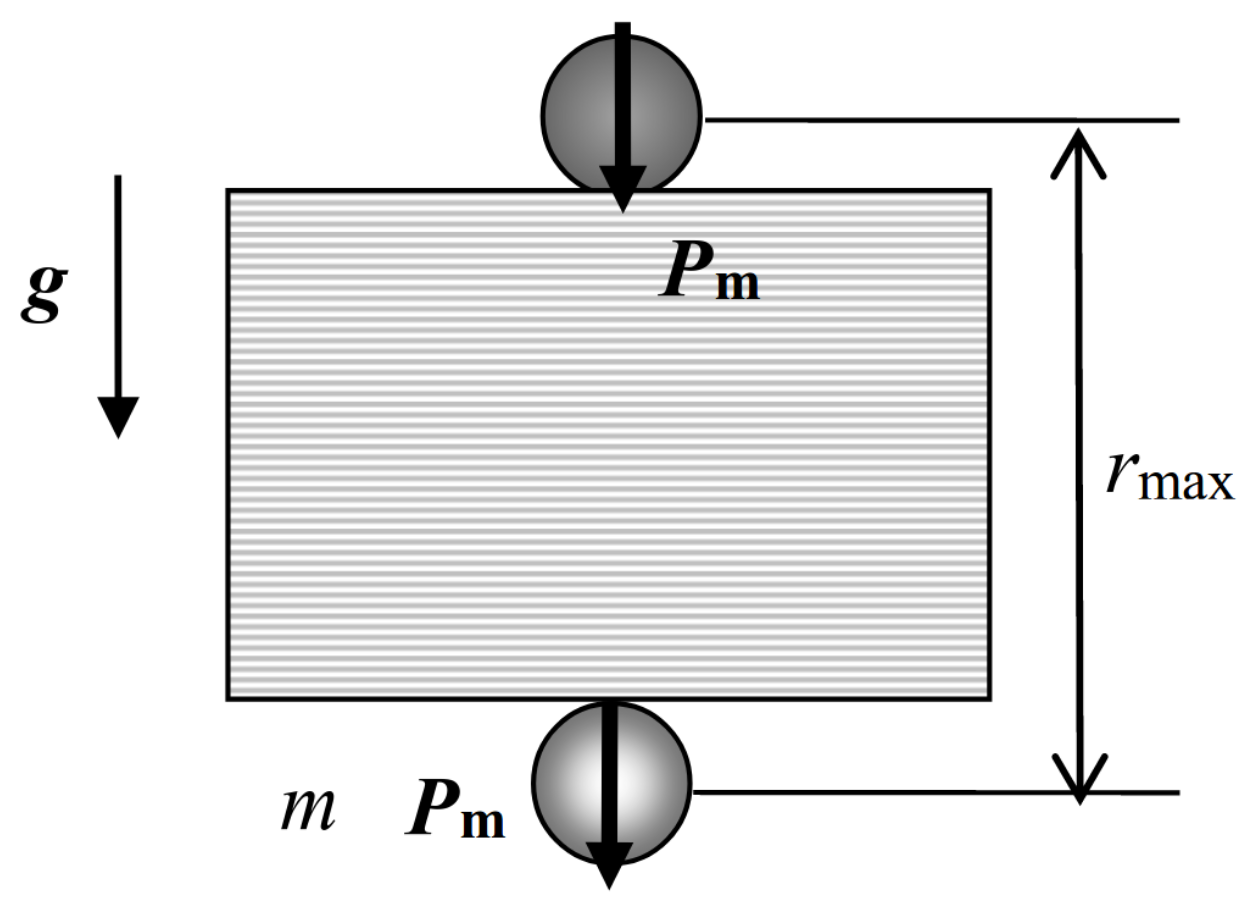
\includegraphics[width = 0.5\linewidth]{zadanie_1.png}
	\caption{Определение  магнитного  момента  шариков  по силе тяжести.}
	\end{figure}
		\begin{figure}[H]
	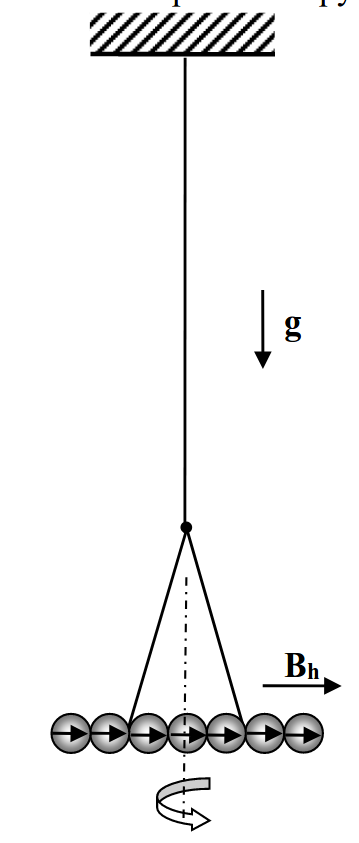
\includegraphics[width = 0.41\linewidth]{zadanie_2.png}
	\caption{Определение  горизонтальной составляющей поля Земли.}
	\end{figure}		\begin{figure}[H]
	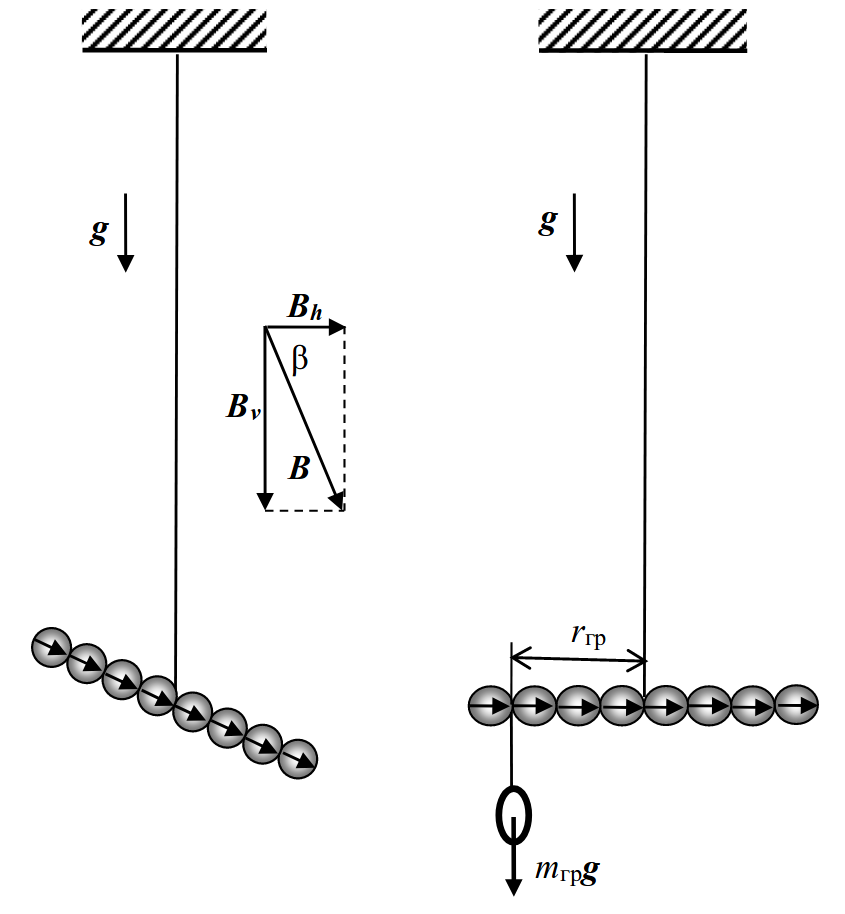
\includegraphics[width = 0.5\linewidth]{zadanie_3.png}
	\caption{Определение  вертикальной составляющей поля Земли.}
	\end{figure}
	\section*{Теоретическая часть}
	\textbf{Точечный магнитный диполь.}
	
	Простейший магнитный диполь может быть образован витком с током или постоянным магнитом. По определению, магнитный момент $\vec P_m$ тонкого витка $S$ c током $I$ равен:
\[
	\vec P_m = (I/c)\, \vec S = (I/c) S\, \vec n,
\]
где $c$ --- скорость света в вакууме, $\vec S = S \, \vec n$ --- вектор площади контура, образующий с направлением тока правовинтовую систему, $\vec n$ --- единичный вектор нормали к площадке $S$ (это же направление $\vec P_m$ принимается за направление $S \longrightarrow N$ от южного ($S$) к северному ($N$) полюсу). Если размеры контура с током или магнитной стрелки малы по сравнению с расстоянием до диполя, то соответствующий магнитный диполь $\vec P_m$ называют элементарным или точечным.

Магнитное поле точечного диполя определяется по формуле, аналогичной формуле для поля элементарного электрического диполя:
\[
	\vec B = 3 (\vec P_m \vec r) \vec r / r^5 - \vec P_m / r^3.
\]
	В магнитном поле с индукцией $\vec B$ на точечный магнитный диполь $\vec P_m$ действует механический момент сил:
\[
	\vec M = \vec P_m \times \vec B.
\]
	Под действием вращающего момента $\vec M$ виток с током или постоянный магнит поворачивается так, чтобы его магнитный момент выстроился вдоль вектора индукции магнитного поля. Это --- положение устойчивого равновесия: при отклонении от этого положения возникает механический момент внешних сил, возвращающий диполь к положению равновесия. В положении, когда $\vec P_m$ и $\vec B$ параллельны, но направлены противоположно друг другу, также имеет место равновесие ($M = 0$), но такое равновесие неустойчиво: малейшее отклонение от этого положения приведёт к появлению момента сил, стремящихся отклонить диполь ещё дальше от начальногомагнитный момент шарика положения.
	
	Магнитный диполь в магнитном поле обладает энергией:
	\[
		W = - (\vec P_m , \vec B).
	\]
	Из этой формулы следует, что энергия диполя в поле минимальна и равна $W_{min} = - P_m B$ при сонаправленных векторах $\vec P_m \upuparrows \vec B$ (угол $\theta$ между $\vec P_m$ и $\vec B$ равен нулю), т. е., как и следовало ожидать, в положении устойчивого равновесия.
	
	Обратим внимание на то, что формула для энергии диполя в магнитном поле очень удобна для выяснения единиц измерения магнитного диполя $\vec P_m$, причём, как в системе СИ, так и в системе СГСЭ, т. к. в обеих системах единиц формулы для энергии диполя выглядит одиаково:
	
	\quad в системе СИ размерность $[P_m] = [W]/[B] = \text{Дж/Тл}$;
	
	\quad в системе СГСЭ размерность $[P_m] = [W]/[B] = \text{эрг/Гс}$.

	В неоднородном поле на точечный магнитный диполь, кроме момента сил, действует ещё и сила:
\[
	\vec F = (\vec P_m, \vec \Delta) \vec E.
\]
Используя формулы для момента силы, силы и энергии, не сложно выяснить, как ведёт себя свободный магнитный диполь в неоднородном магнитном поле: он выстраивается вдоль силовых линий магнитного поля и, кроме того, под действием результирующей силы, возникающей из-за неоднородности поля, втягивается в область более сильного магнитного поля, т.е. в область, где он обладает меньшей энергией.

Зная магнитные моменты $P_1$ и $P_2$ двух небольших постоянных магнитов, можно рассчитать силу их взаимодействия. Если магнитные моменты $P_1 = P_2 = P_m$ двух одинаковых небольших магнитов направлены вдоль соединяющей их прямой, а расстояние между ними равно $r$, то магниты взаимодействуют с силой:
\[
	F = P_m \partial B / \partial r = P_m \partial(2P_m / r^3)/\partial r = - 6 P_m^2 / r^4.
\]
Магниты притягиваются, если их магнитные моменты сонаправлены ($\vec P_1 \upuparrows \vec P_2$) и отталкиваются, если моменты направлены противоположно друг другу ($\vec P_1 \uparrow \downarrow \vec P_2$).

Если магнитные моменты направлены перпендикулярно соединяющей их прямой, то сила их взаимодействия окажется в два раза меньшей: $F = 3p^2 / r^4$ (в этом случае диполи притягиваются при $\vec P_1 \uparrow \downarrow \vec P_2$ и отталкиваются при $\vec P_1 \uparrow \uparrow \vec P_2$).
	
	\textbf{Неодимовые магнитные шары.}
	
	В настоящей работе используются неодимовые магниты шарообразной формы.
	
	Для нас важно то, что:
		1) шары намагничены однородно;
		2) Вещество, из которого изготовлены магниты, является магнитожёстким материалом.
		Магнитное поле однородно намагниченного шара радиуса $R$ на расстояниях $r \ge R$ от центра шара совпадает с полем точечного магнитного диполя $\vec P_m$, равного полному магнитному моменту шара и расположенного в центре (можно сказать, что внутри ($r < R$) такого шара поле однородно и равно $B_0 = 2 P_m / R^3$)
		
		Магнитожёсткость материала означает, что магнитные моменты шаров в нашей работе не изменяются под действием внешних магнитных полей, т. е. шар ведёт как жёсткий диполь. Поэтому, при расчетах можно считать, что шары взаимодействуют как жёсткие точечные магнитные диполи, расположенные в центрах шаров.
		
		Полный магнитный момент $\vec P_m$ постоянного магнита определяется намагниченностью $\vec p_m$ вещества, из которого он изготовлен. По определению, намагниченность --- это магнитный момент единицы объёма. ДЛя однородно намагниченного шара намагниченность, очевидно, равна:
\[
	\vec p_m = \vec P_m / V,
\]		
	где $V$ --- объём шара.
		 Намагниченность --- важная характеристика вещества постоянных магнитов, определяющая, в частности, величину остаточной магнитной индукции $B_r = 4 \pi p_m$ (остаточная индукция $B_r$ --- одна из величин, которая, как правило, указывается в справочниках по магнитожёстким материалам).
		 
		 Не сложно показать, что индукция магнитного поля $\vec B_p$ на полюсах однородно намагниченного шара связана с величиной намагниченности $\vec p_m$ и остаточной магнитной индукцией $\vec B_r$ формулой:
\[
	\vec B_p = (8 \pi / 3) \vec p_m = (2 / 3) \vec B_r.
\]
		
	\textbf{Экспериментальное  определение  величины  магнитного момента магнитных шариков.}	
	
Величину магнитного момента $P_m$ одинаковых шариков можно рассчитать, зная их массу $m$ и определив максимальное расстояние $r_{max}$, на котором они ещё удерживают друг друга в поле тяжести (см. рис.1). При максимальном расстоянии сила тяжести шариков равна силе их магнитного притяжения:
\[
	6 P_m^2 / r_{max}^4 = mg, \quad P_m = \sqrt{\frac{mgr_{max}^4}{6}}.
\]
По величине магнитного момента $P_m$ можно рассчитать величину индукции магнитного поля вблизи любой точки на поверхности шара радиуса $R$. Максимальная величина индукции наблюдаются на полюсах:
\[
	\vec B_p = 2 \vec P_m / R^3.
\]
 \textbf{Измерение горизонтальной составляющей индукции магнитного поля Земли.}
 
 Магнитное поле Земли в настоящей работе определяется по периоду крутильных колебаний магнитной стрелки вокруг вертикальной оси.
 
 <<Магнитная стрелка>> образована из сцепленных друг с другом противоположными полюсами шариков и с помощью $\wedge$-образного подвеса  подвешена  в  горизонтальном  положении (см. рис. 2). Магнитные моменты шариков направлены в одну сторону  вдоль  оси  <<стрелки>>.
 Под действием вращательного момента $\vec M = \vec P_0 \times \vec B$ магнитный момент <<стрелки>> $\vec P_0$ выстроится вдоль горизонтальной составляющей магнитного поля Земли $\vec B_h$ в направлении Юг $\rightarrow$ Север. При отклонении <<стрелки>> на угол $\theta$ от равновесного положения в горизонтальной плоскости возникают крутильные колебания вокруг вертикальной оси, проходящей через середину стрелки.Если пренебречь упругостью нити, то уравнение крутильных колебаний такого  маятника определяется возвращающим  моментом  сил 
 $M = - P_0 B_h \sin \theta$, дейсвующим на <<стрелку>> со стороны магнитного поля Земли, и моментом инерции $I_n$ <<стрелки>> относительно оси вращения.
 
 При малых амплитудах $(\sin \theta \approx \theta)$ уравнение колебаний <<стрелки>> имеет вид:
\[
	I_n d^2 \theta / dt^2 = - P_0 B_h 	\theta, \quad \text{или} \quad I_n \ddot \theta 	+ P_0 B_h \theta = 0.
\]
Период колебаний:
\[
	T = 2 \pi \sqrt{I_n / P_0 B_h} = 2 \pi \sqrt{I_n / n P_m B_h},
\]
где $P_0 = nP_m$ --- полный магнитный момент магнитной <<стрелки>>, составленной
из $n$ шариков.

Момент инерции <<стрелки>>, сотоящей из $n$ шариков, как не сложно убедиться, с хорошей точностью равен моменту инерции тонкого однородного стержня массой $m_{ст} = nm$ и длиной $l_{ст} = nd$:
\[
	I_n = (1/12)m_{\text{ст}}l_{\text{ст}}^2 = (1/12)nm(nd)^2 = (1/12)n^3md^2.
\]
Даже для трёх шариков момент инерции, рассчитанный по приближённой формуле, отличается от точного результата примерно на 2 \%, а для $n \ge 5$ --- различие не превышает процента; если же учесть, что $T \sim \sqrt{I_n}$, то для всех $n \ge 3$ погрешность наших расчётов для периода колебаний $T$ не превысит процента, что освобождает нас от необходимости вводить поправочные коэффиценты.

Таким образом, в нашем приближении период колебаний маятника оказывается пропорциональным числу шаров $n$, составляющих <<стрелку>>:
\[
	T(n) = 2 \pi \sqrt{I_n / n P_m B_h} = 
	\]
	\[
	= 2 \pi \sqrt{n^3 m d^2 / 12 n P_m B_h}
	 = \pi n \sqrt{m d^2 / 3 P_m B_h} = kn,
\]

где $k = \pi \sqrt{m d^2 / 3 P_m B_h}$.

 При выводе этой формулы предполагалось, что магнитный момент --- величина аддитивная: полный магнитный момент системы магнитов (<<стрелки>>)равен векторной сумме магнитных моментов шариков, составляющих <<стрелку>>. Экспериментальное подтверждение этой зависимости $(T \sim n)$ будет являться косвенным доказательством наших предположений о магнитожёсткости материала магнитов и, соответственно, свойства аддитивности магнитных моментов шаров.
 
\textbf{Измерение вертикальной составляющей индукции магнитного поля Земли. Магнитное наклонение.} 

Для измерения вертикальной $B_v$ составляющей вектора индукции поля Земли используется та же установка, что и для измерения горизонтальной составляющей  с  тем  лишь  отличием, что магнитная <<стрелка>> подвешивается на нити без $\wedge$-образного подвеса. В этом случае магнитная  <<стрелка>>,  составленная  из  чётного  числа шариков и подвешенная на тонкой нити за середину, расположится не горизонтально, а под некоторым, отличным от нуля, углом к горизонту (см. рис. 3, слева). Это связано с тем, что вектор $\vec B$  индукции магнитного поля Земли в общем случае  не  горизонтален,  а  образует  с  горизонтом угол $\beta$, зависящим от географической широты $\phi$ места,  где  проводится  опыт. Величина  угла $\beta$ называется магнитным наклонением.

 С помощью  небольшого  дополнительного грузика  <<стрелку>>  можно <<выровнять>>, расположив её горизонтально (см.рис. 3, справа): в этом случае момент силы тяжести груза относительно точки  подвеса будет  равен моменту сил,  действующих на <<стрелку>> со стороны магнитного поля  Земли. Если масса уравновешивающего груза равна $m_\text{гр}$, плечо силы тяжести $r_\text{гр}$, а полный магнитный момент <<стрелки>> $P_0 = n P_m$, то в равновесии: 
\[
	m_\text{гр} g r_\text{гр} = P_0 B_v = n P_m B_v,
\]
где $B_v$ --- вертикальная составляющая поля Земли.
Видно, что момент $M(n)$ силы тяжести уравновешивающего груза пропорционален числу $n$ шариков, образующих магнитную <<стрелку>>:
\[
	M(n) = An, \quad A = P_m B_v.
\]
\section*{Обработка результатов измерений}
\textbf{Определение магнитного момента, намагниченности и остаточной магнитной индукции вещества магнитных шариков.}

\begin{table}[H]

	\centering
	\begin{tabular}{|c|c|c|} \hline
		$N$ &  $m, 10^{-3}\ \text{г}$ & $d, 10^{-2}\ \text{см}$ \\\hline
		1 &  863 &  61 \\\hline
		2 &  848 &  62 \\\hline
		3 &  857 &  63 \\\hline
		4 &  846 &  62 \\\hline
		5 &  838 &  60 \\\hline
		6 &  850 &  61 \\\hline
		7 &  853 &  62 \\\hline
		8 &  842 &  61 \\\hline
		9 &  844 &  63 \\\hline
		10 &  853 &  62 \\\hline
		11 &  847 &  61 \\\hline
		12 &  848 &  60 \\\hline
	\end{tabular}	
	\caption{Измерения первого задания.}
\end{table}
Проложим между двумя магнитными шариками брусок из немагнитного материала; выясним максимальное расстояние, при котором шарики удерживают друг друга в поле Земли с учётом случайной погрешности:
\[
	r_{max} = 2,5 \pm 0,1\ \text{см}.
\]
Рассчитаем величину $p_m$:
\[
	P_m = \sqrt{\frac{mgr_{max}^4}{6}} = 73 \pm 2\ \frac{\text{эрг}}{\text{Гс}}
\]
\[
	p_m = \frac{P_m}{V} = 600 \pm 30 \frac{\text{эрг}}{\text{Гс}\cdot \text{см}^3}
\]
Рассчитаем величину $B_p$  и $B_r$ материала, из которого изготовлен шарик:
\[
	B_p = 2 P_m / R^3 = 5,0 \pm 0,2 \ \text{кГс}.
\]
\[
	B_r = 4 \pi p_m = 7,5 \pm 0,3 \ \text{кГс}; \quad B_{r_\text{табл}} = 11,5 \text{---} 14\ \text{кГс}
\]
\textbf{Определение горизонтальной составляющей магнитного поля Земли.}

Измерим зависимость периода $T$ крутильных колебаний <<стрелки>> от количества магнитных шариков $n$, составляющих <<стрелку>>, померив количество периодов $k$ за время $t$:
\begin{table}[H]
	\centering
	\begin{tabular}{|c|c|} \hline
$n$ &     $T, c$ \\\hline
3 &  0,86 \\\hline
4 &  1,09 \\\hline
5 &  1,32 \\\hline
6 &  1,53 \\\hline
7 &  1,78 \\\hline
8 &  2,05 \\\hline
9 &  2,31 \\\hline
10 &  2,58 \\\hline
11 &  2,86 \\\hline
12 &  3,14 \\\hline
	\end{tabular}
	\caption{Измерения второго задания.}
\end{table}
Построим график зависимости $T$ от $n$:
\begin{figure}[H]
	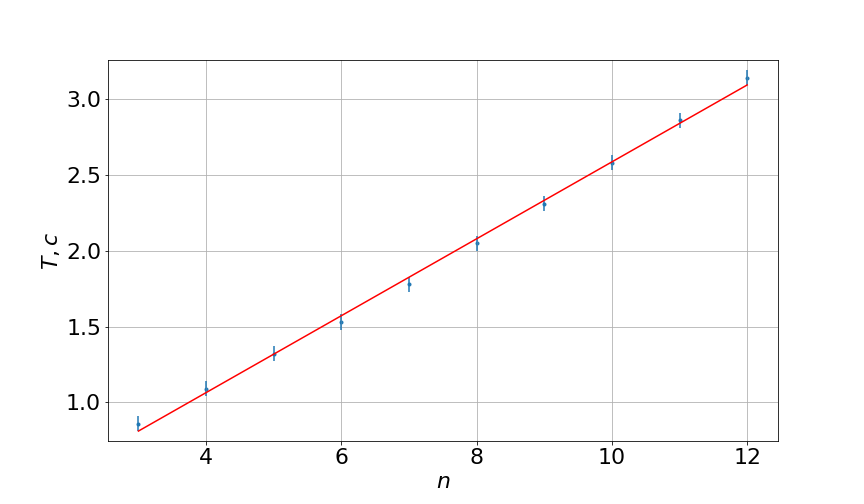
\includegraphics[width = 0.9\linewidth]{2.png}
	\caption{График зависимости $T = kn$}
	\end{figure}
\[
	k = 0,253 \pm 0,018
\]
Вычислим величину горизонтальной составляющей магнитного поля Земли:
\[
	B_h = \frac{\pi^2 m d^2}{2 k^2 P_m} = 0,227 \pm 0,024\ \text{Гс}
\]
Рассчитаем моменты сил тяжести для разного количества шариков:
\[
	M = m\cdot g \cdot d \cdot (\frac{N}{2} - 1)
\]
\begin{table}[H]
	\centering
	\begin{tabular}{|c|c|c|c|c|c|} \hline
	$N,\ \text{шт}$	 & 4 & 6 & 8 & 10 & 12					\\\hline
	$M, \frac{\text{г} \cdot \text{см}^3}{\text{c}^2}$	& 172,98 & 314,61 & 428,31 & 547,25 & 641,88	\\\hline
\end{tabular}
\end{table}
Построим график момента силы тяжести $M$ от числа шариков $n$ для нахождения вертикальной составляющей магнитного поля Земли:
\begin{figure}[H]
	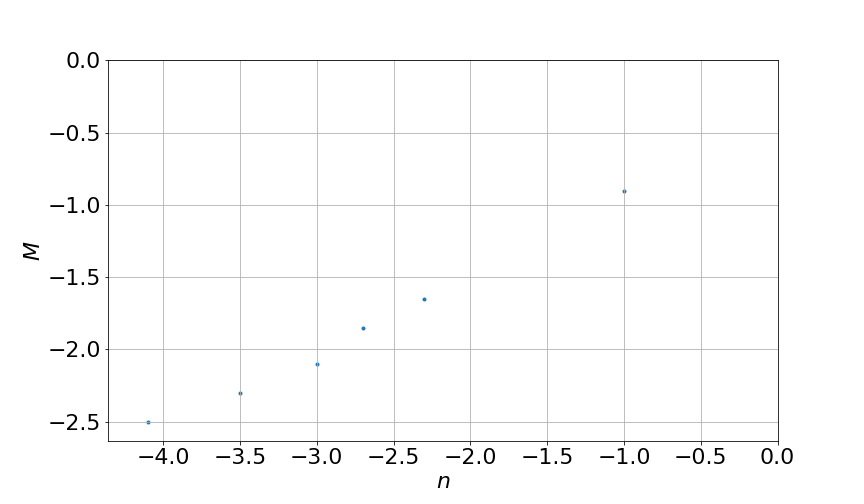
\includegraphics[width = 1.0\linewidth]{3.png}
	\caption{График зависимости $M = An$}
	\end{figure}
\[
	A = 48 \pm 4
\]
\[
	B_v = \frac{A}{P_m} = 0,66 \pm 0,10\ \text{Гс}
\]
Магнитное поле Земли:
\[
	B = 0,70 \pm 0.13\ \text{Гс}
\]
\section*{Вывод}
Полученное с помощью магнитных неодимовых шариков магнитное поле Земли с учетом погрешности совпадает с табличным: $B_\text{табл} = 0.25 \text{---} 0.65\ \text{Гс}$, что можно с некоторой степенью сказать и о остаточной магнитной индукции, однако расхождения с табличными данными получились заметными из-за большой случайной погрешности.

\end{document}